\title{Trabalho 2 de EA876 - Blur filter}
\author{
        Maruan Bakri Ottoni \\
                FEEC\\
        UNICAMP\\
        Campinas, \underline{Brasil}
}
\date{\today}
\documentclass[12pt]{article}
\usepackage[dvipsnames]{xcolor}
\usepackage{fancyvrb}
\usepackage{float}
\usepackage{graphicx}
\RecustomVerbatimCommand{\VerbatimInput}{VerbatimInput}%
{fontsize=\footnotesize,
 frame=lines,
 framesep=2em,
 rulecolor=\color{Gray},
 label=\fbox{\color{Black}data.txt},
 labelposition=topline,
 commandchars=\|\(\),
 commentchar=*
}

\begin{document}
\maketitle

\section{Sys Time}
    \begin{figure}[H]
        \caption{Grafico de sys time para uma linha de execucao.}
        \centering
        \includegraphics[width=8cm]{doc/sys_simples.png}
    \end{figure}
    \VerbatimInput{doc/sys_simples.log}

    \begin{figure}[H]
        \caption{Grafico de sys time para multiprocess.}
        \centering
        \includegraphics[width=8cm]{doc/sys_processos.png}
    \end{figure}
    \VerbatimInput{doc/sys_processos.log}

    \begin{figure}[H]
        \caption{Grafico de sys time para multithread.}
        \centering
        \includegraphics[width=8cm]{doc/sys_threads.png}
    \end{figure}
    \VerbatimInput{doc/sys_threads.log}

\section{User time}
    \begin{figure}[H]
        \caption{Grafico de user time para uma linha de execucao.}
        \centering
        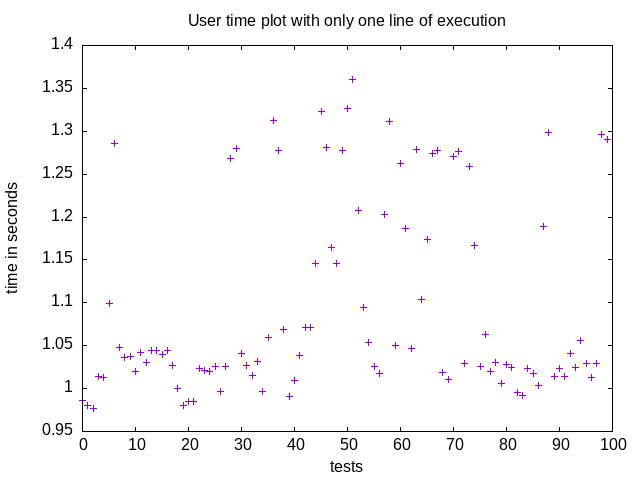
\includegraphics[width=8cm]{doc/user_simples.png}
    \end{figure}
    \VerbatimInput{doc/user_simples.log}

    \begin{figure}[H]
        \caption{Grafico de user time para multiprocess.}
        \centering
        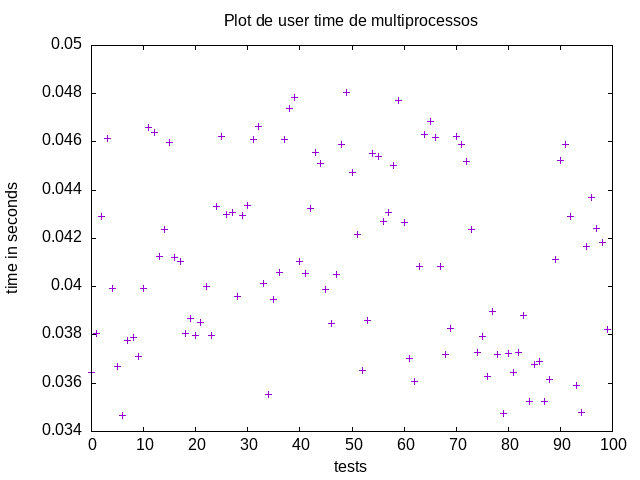
\includegraphics[width=8cm]{doc/user_processos.png}
    \end{figure}
    \VerbatimInput{doc/user_processos.log}

    \begin{figure}[H]
        \caption{Grafico de user time para multithread.}
        \centering
        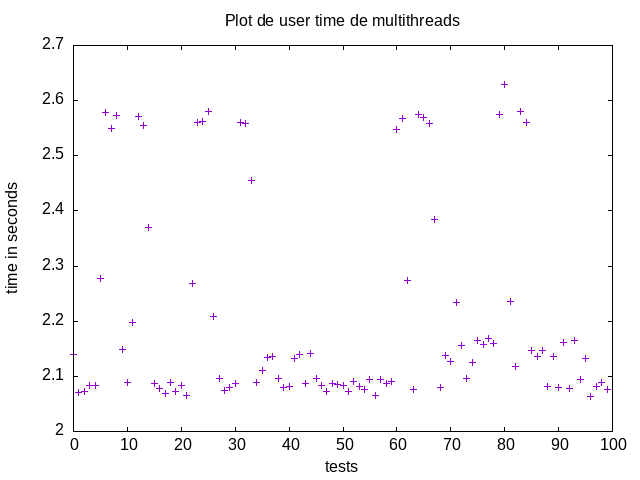
\includegraphics[width=8cm]{doc/user_threads.png}
    \end{figure}
    \VerbatimInput{doc/user_threads.log}


\section{Real Time}\label{results}
    \begin{figure}[H]
        \caption{Grafico de real time para uma linha de execucao.}
        \centering
        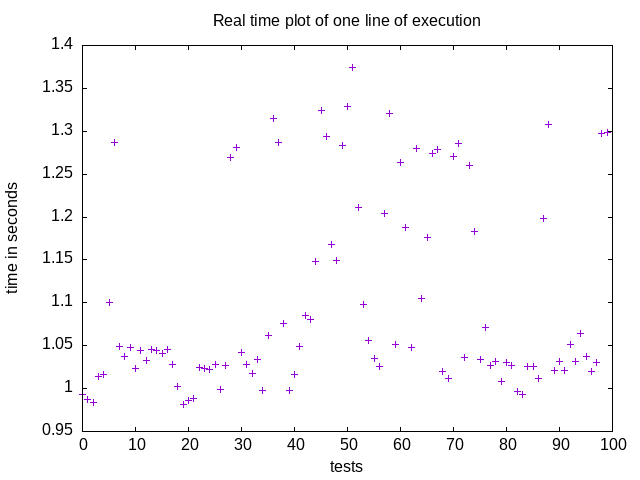
\includegraphics[width=8cm]{doc/real_simples.png}
    \end{figure}
    \VerbatimInput{doc/real_simples.log}

    \begin{figure}[H]
        \caption{Grafico de real time para multiprocess.}
        \centering
        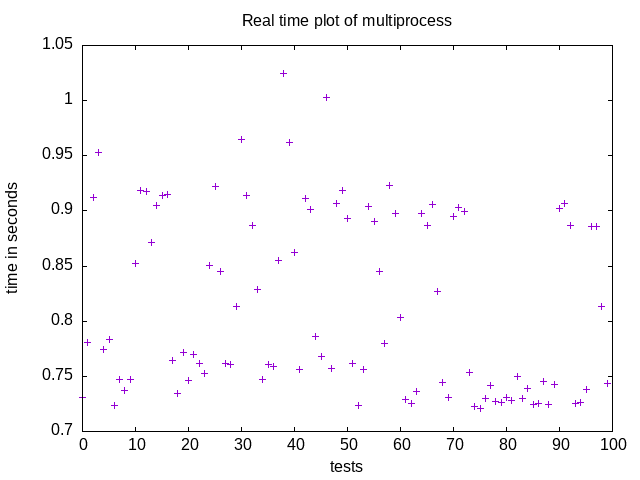
\includegraphics[width=8cm]{doc/real_processos.png}
    \end{figure}
    \VerbatimInput{doc/real_processos.log}

    \begin{figure}[H]
        \caption{Grafico de real time para multithread.}
        \centering
        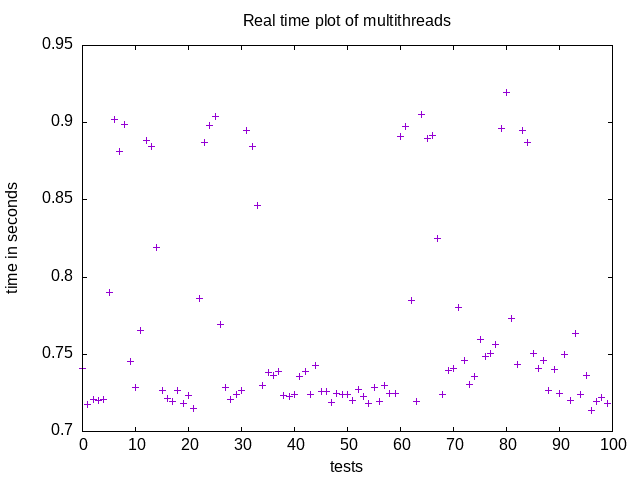
\includegraphics[width=8cm]{doc/real_threads.png}
    \end{figure}
    \VerbatimInput{doc/real_threads.log}

\end{document}
